\documentclass[11pt]{article}
\usepackage[OT4]{fontenc}
\newtheorem{define}{Definition}
\usepackage{graphicx}
\usepackage{subcaption}
\oddsidemargin=0.15in
\evensidemargin=0.15in
\topmargin=-.5in
\textheight=9in
\textwidth=6.25in

\begin{document}
	
%--------------
%% preamble.tex
%% this should be included with a command like
%% %--------------
%% preamble.tex
%% this should be included with a command like
%% %--------------
%% preamble.tex
%% this should be included with a command like
%% \input{preamble.tex}
%% Template based on Aleksander Madry's and Dan Spielman's template

\hbadness=10000
\vbadness=10000

\setlength{\oddsidemargin}{.25in}
\setlength{\evensidemargin}{.25in}
\setlength{\textwidth}{6in}
\setlength{\topmargin}{-0.4in}
\setlength{\textheight}{8.5in}

\newcommand{\handout}[5]{
	\noindent
	\begin{center}
		\framebox{
			\vbox{
				\hbox to 5.78in { {\bf #1}
					\hfill #2 }
				\vspace{4mm}
				\hbox to 5.78in { {\Large \hfill #5  \hfill} }
				\vspace{2mm}
				\hbox to 5.78in { {\it #3 \hfill #4} }
			}
		}
	\end{center}
	\vspace*{4mm}
}

\newcommand{\header}[2]{\handout{NUS CS4243: Computer Vision and Pattern Recognition}{\today}{Lecturer: Angela Yao;}{Students: #1}{#2}}


\newtheorem{theorem}{Theorem}
\newtheorem{corollary}[theorem]{Corollary}
\newtheorem{lemma}[theorem]{Lemma}
\newtheorem{observation}[theorem]{Observation}
\newtheorem{proposition}[theorem]{Proposition}
\newtheorem{definition}[theorem]{Definition}
\newtheorem{claim}[theorem]{Claim}
\newtheorem{fact}[theorem]{Fact}
\newtheorem{assumption}[theorem]{Assumption}

\newcommand{\qed}{\rule{7pt}{7pt}}
\newcommand{\dis}{\mathop{\mbox{\rm d}}\nolimits}
\newcommand{\per}{\mathop{\mbox{\rm per}}\nolimits}
\newcommand{\area}{\mathop{\mbox{\rm area}}\nolimits}
\newcommand{\cw}{\mathop{\rm cw}\nolimits}
\newcommand{\ccw}{\mathop{\rm ccw}\nolimits}
\newcommand{\DIST}{\mathop{\mbox{\rm DIST}}\nolimits}
\newcommand{\OP}{\mathop{\mbox{\it OP}}\nolimits}
\newcommand{\OPprime}{\mathop{\mbox{\it OP}^{\,\prime}}\nolimits}
\newcommand{\ihat}{\hat{\imath}}
\newcommand{\jhat}{\hat{\jmath}}
\newcommand{\abs}[1]{\mathify{\left| #1 \right|}}

\newenvironment{proof}{\noindent{\bf Proof}\hspace*{1em}}{\qed\bigskip}
\newenvironment{proof-sketch}{\noindent{\bf Sketch of Proof}\hspace*{1em}}{\qed\bigskip}
\newenvironment{proof-idea}{\noindent{\bf Proof Idea}\hspace*{1em}}{\qed\bigskip}
\newenvironment{proof-of-lemma}[1]{\noindent{\bf Proof of Lemma #1}\hspace*{1em}}{\qed\bigskip}
\newenvironment{proof-attempt}{\noindent{\bf Proof Attempt}\hspace*{1em}}{\qed\bigskip}
\newenvironment{proofof}[1]{\noindent{\bf Proof}
of #1:\hspace*{1em}}{\qed\bigskip}
\newenvironment{remark}{\noindent{\bf Remark}\hspace*{1em}}{\bigskip}

% \makeatletter
% \@addtoreset{figure}{section}
% \@addtoreset{table}{section}
% \@addtoreset{equation}{section}
% \makeatother

\newcommand{\FOR}{{\bf for}}
\newcommand{\TO}{{\bf to}}
\newcommand{\DO}{{\bf do}}
\newcommand{\WHILE}{{\bf while}}
\newcommand{\AND}{{\bf and}}
\newcommand{\IF}{{\bf if}}
\newcommand{\THEN}{{\bf then}}
\newcommand{\ELSE}{{\bf else}}

% \renewcommand{\thefigure}{\thesection.\arabic{figure}}
% \renewcommand{\thetable}{\thesection.\arabic{table}}
% \renewcommand{\theequation}{\thesection.\arabic{equation}}

\makeatletter
\def\fnum@figure{{\bf Figure \thefigure}}
\def\fnum@table{{\bf Table \thetable}}
\long\def\@mycaption#1[#2]#3{\addcontentsline{\csname
  ext@#1\endcsname}{#1}{\protect\numberline{\csname 
  the#1\endcsname}{\ignorespaces #2}}\par
  \begingroup
    \@parboxrestore
    \small
    \@makecaption{\csname fnum@#1\endcsname}{\ignorespaces #3}\par
  \endgroup}
\def\mycaption{\refstepcounter\@captype \@dblarg{\@mycaption\@captype}}
\makeatother

\newcommand{\figcaption}[1]{\mycaption[]{#1}}
\newcommand{\tabcaption}[1]{\mycaption[]{#1}}
\newcommand{\head}[1]{\chapter[Lecture \##1]{}}
\newcommand{\mathify}[1]{\ifmmode{#1}\else\mbox{$#1$}\fi}
%\renewcommand{\Pr}[1]{\mathify{\mbox{Pr}\left[#1\right]}}
%\newcommand{\Exp}[1]{\mathify{\mbox{Exp}\left[#1\right]}}
\newcommand{\bigO}O
\newcommand{\set}[1]{\mathify{\left\{ #1 \right\}}}
\def\half{\frac{1}{2}}

\newcommand{\fig}[4]{
        \begin{figure}
        \setlength{\epsfysize}{#2}
        \vspace{3mm}
        \centerline{\epsfbox{#4}}
        \caption{#3} \label{#1}
        \end{figure}
        }

\newcommand{\ord}{{\rm ord}}

\providecommand{\norm}[1]{\lVert #1 \rVert}
\newcommand{\embed}{{\rm Embed}}
\newcommand{\qembed}{\mbox{$q$-Embed}}
\newcommand{\calh}{{\cal H}}
\newcommand{\lp}{{\rm LP}}

%% Template based on Aleksander Madry's and Dan Spielman's template

\hbadness=10000
\vbadness=10000

\setlength{\oddsidemargin}{.25in}
\setlength{\evensidemargin}{.25in}
\setlength{\textwidth}{6in}
\setlength{\topmargin}{-0.4in}
\setlength{\textheight}{8.5in}

\newcommand{\handout}[5]{
	\noindent
	\begin{center}
		\framebox{
			\vbox{
				\hbox to 5.78in { {\bf #1}
					\hfill #2 }
				\vspace{4mm}
				\hbox to 5.78in { {\Large \hfill #5  \hfill} }
				\vspace{2mm}
				\hbox to 5.78in { {\it #3 \hfill #4} }
			}
		}
	\end{center}
	\vspace*{4mm}
}

\newcommand{\header}[2]{\handout{NUS CS4243: Computer Vision and Pattern Recognition}{\today}{Lecturer: Angela Yao;}{Students: #1}{#2}}


\newtheorem{theorem}{Theorem}
\newtheorem{corollary}[theorem]{Corollary}
\newtheorem{lemma}[theorem]{Lemma}
\newtheorem{observation}[theorem]{Observation}
\newtheorem{proposition}[theorem]{Proposition}
\newtheorem{definition}[theorem]{Definition}
\newtheorem{claim}[theorem]{Claim}
\newtheorem{fact}[theorem]{Fact}
\newtheorem{assumption}[theorem]{Assumption}

\newcommand{\qed}{\rule{7pt}{7pt}}
\newcommand{\dis}{\mathop{\mbox{\rm d}}\nolimits}
\newcommand{\per}{\mathop{\mbox{\rm per}}\nolimits}
\newcommand{\area}{\mathop{\mbox{\rm area}}\nolimits}
\newcommand{\cw}{\mathop{\rm cw}\nolimits}
\newcommand{\ccw}{\mathop{\rm ccw}\nolimits}
\newcommand{\DIST}{\mathop{\mbox{\rm DIST}}\nolimits}
\newcommand{\OP}{\mathop{\mbox{\it OP}}\nolimits}
\newcommand{\OPprime}{\mathop{\mbox{\it OP}^{\,\prime}}\nolimits}
\newcommand{\ihat}{\hat{\imath}}
\newcommand{\jhat}{\hat{\jmath}}
\newcommand{\abs}[1]{\mathify{\left| #1 \right|}}

\newenvironment{proof}{\noindent{\bf Proof}\hspace*{1em}}{\qed\bigskip}
\newenvironment{proof-sketch}{\noindent{\bf Sketch of Proof}\hspace*{1em}}{\qed\bigskip}
\newenvironment{proof-idea}{\noindent{\bf Proof Idea}\hspace*{1em}}{\qed\bigskip}
\newenvironment{proof-of-lemma}[1]{\noindent{\bf Proof of Lemma #1}\hspace*{1em}}{\qed\bigskip}
\newenvironment{proof-attempt}{\noindent{\bf Proof Attempt}\hspace*{1em}}{\qed\bigskip}
\newenvironment{proofof}[1]{\noindent{\bf Proof}
of #1:\hspace*{1em}}{\qed\bigskip}
\newenvironment{remark}{\noindent{\bf Remark}\hspace*{1em}}{\bigskip}

% \makeatletter
% \@addtoreset{figure}{section}
% \@addtoreset{table}{section}
% \@addtoreset{equation}{section}
% \makeatother

\newcommand{\FOR}{{\bf for}}
\newcommand{\TO}{{\bf to}}
\newcommand{\DO}{{\bf do}}
\newcommand{\WHILE}{{\bf while}}
\newcommand{\AND}{{\bf and}}
\newcommand{\IF}{{\bf if}}
\newcommand{\THEN}{{\bf then}}
\newcommand{\ELSE}{{\bf else}}

% \renewcommand{\thefigure}{\thesection.\arabic{figure}}
% \renewcommand{\thetable}{\thesection.\arabic{table}}
% \renewcommand{\theequation}{\thesection.\arabic{equation}}

\makeatletter
\def\fnum@figure{{\bf Figure \thefigure}}
\def\fnum@table{{\bf Table \thetable}}
\long\def\@mycaption#1[#2]#3{\addcontentsline{\csname
  ext@#1\endcsname}{#1}{\protect\numberline{\csname 
  the#1\endcsname}{\ignorespaces #2}}\par
  \begingroup
    \@parboxrestore
    \small
    \@makecaption{\csname fnum@#1\endcsname}{\ignorespaces #3}\par
  \endgroup}
\def\mycaption{\refstepcounter\@captype \@dblarg{\@mycaption\@captype}}
\makeatother

\newcommand{\figcaption}[1]{\mycaption[]{#1}}
\newcommand{\tabcaption}[1]{\mycaption[]{#1}}
\newcommand{\head}[1]{\chapter[Lecture \##1]{}}
\newcommand{\mathify}[1]{\ifmmode{#1}\else\mbox{$#1$}\fi}
%\renewcommand{\Pr}[1]{\mathify{\mbox{Pr}\left[#1\right]}}
%\newcommand{\Exp}[1]{\mathify{\mbox{Exp}\left[#1\right]}}
\newcommand{\bigO}O
\newcommand{\set}[1]{\mathify{\left\{ #1 \right\}}}
\def\half{\frac{1}{2}}

\newcommand{\fig}[4]{
        \begin{figure}
        \setlength{\epsfysize}{#2}
        \vspace{3mm}
        \centerline{\epsfbox{#4}}
        \caption{#3} \label{#1}
        \end{figure}
        }

\newcommand{\ord}{{\rm ord}}

\providecommand{\norm}[1]{\lVert #1 \rVert}
\newcommand{\embed}{{\rm Embed}}
\newcommand{\qembed}{\mbox{$q$-Embed}}
\newcommand{\calh}{{\cal H}}
\newcommand{\lp}{{\rm LP}}

%% Template based on Aleksander Madry's and Dan Spielman's template

\hbadness=10000
\vbadness=10000

\setlength{\oddsidemargin}{.25in}
\setlength{\evensidemargin}{.25in}
\setlength{\textwidth}{6in}
\setlength{\topmargin}{-0.4in}
\setlength{\textheight}{8.5in}

\newcommand{\handout}[5]{
	\noindent
	\begin{center}
		\framebox{
			\vbox{
				\hbox to 5.78in { {\bf #1}
					\hfill #2 }
				\vspace{4mm}
				\hbox to 5.78in { {\Large \hfill #5  \hfill} }
				\vspace{2mm}
				\hbox to 5.78in { {\it #3 \hfill #4} }
			}
		}
	\end{center}
	\vspace*{4mm}
}

\newcommand{\header}[2]{\handout{NUS CS4243: Computer Vision and Pattern Recognition}{\today}{Lecturer: Angela Yao;}{Students: #1}{#2}}


\newtheorem{theorem}{Theorem}
\newtheorem{corollary}[theorem]{Corollary}
\newtheorem{lemma}[theorem]{Lemma}
\newtheorem{observation}[theorem]{Observation}
\newtheorem{proposition}[theorem]{Proposition}
\newtheorem{definition}[theorem]{Definition}
\newtheorem{claim}[theorem]{Claim}
\newtheorem{fact}[theorem]{Fact}
\newtheorem{assumption}[theorem]{Assumption}

\newcommand{\qed}{\rule{7pt}{7pt}}
\newcommand{\dis}{\mathop{\mbox{\rm d}}\nolimits}
\newcommand{\per}{\mathop{\mbox{\rm per}}\nolimits}
\newcommand{\area}{\mathop{\mbox{\rm area}}\nolimits}
\newcommand{\cw}{\mathop{\rm cw}\nolimits}
\newcommand{\ccw}{\mathop{\rm ccw}\nolimits}
\newcommand{\DIST}{\mathop{\mbox{\rm DIST}}\nolimits}
\newcommand{\OP}{\mathop{\mbox{\it OP}}\nolimits}
\newcommand{\OPprime}{\mathop{\mbox{\it OP}^{\,\prime}}\nolimits}
\newcommand{\ihat}{\hat{\imath}}
\newcommand{\jhat}{\hat{\jmath}}
\newcommand{\abs}[1]{\mathify{\left| #1 \right|}}

\newenvironment{proof}{\noindent{\bf Proof}\hspace*{1em}}{\qed\bigskip}
\newenvironment{proof-sketch}{\noindent{\bf Sketch of Proof}\hspace*{1em}}{\qed\bigskip}
\newenvironment{proof-idea}{\noindent{\bf Proof Idea}\hspace*{1em}}{\qed\bigskip}
\newenvironment{proof-of-lemma}[1]{\noindent{\bf Proof of Lemma #1}\hspace*{1em}}{\qed\bigskip}
\newenvironment{proof-attempt}{\noindent{\bf Proof Attempt}\hspace*{1em}}{\qed\bigskip}
\newenvironment{proofof}[1]{\noindent{\bf Proof}
of #1:\hspace*{1em}}{\qed\bigskip}
\newenvironment{remark}{\noindent{\bf Remark}\hspace*{1em}}{\bigskip}

% \makeatletter
% \@addtoreset{figure}{section}
% \@addtoreset{table}{section}
% \@addtoreset{equation}{section}
% \makeatother

\newcommand{\FOR}{{\bf for}}
\newcommand{\TO}{{\bf to}}
\newcommand{\DO}{{\bf do}}
\newcommand{\WHILE}{{\bf while}}
\newcommand{\AND}{{\bf and}}
\newcommand{\IF}{{\bf if}}
\newcommand{\THEN}{{\bf then}}
\newcommand{\ELSE}{{\bf else}}

% \renewcommand{\thefigure}{\thesection.\arabic{figure}}
% \renewcommand{\thetable}{\thesection.\arabic{table}}
% \renewcommand{\theequation}{\thesection.\arabic{equation}}

\makeatletter
\def\fnum@figure{{\bf Figure \thefigure}}
\def\fnum@table{{\bf Table \thetable}}
\long\def\@mycaption#1[#2]#3{\addcontentsline{\csname
  ext@#1\endcsname}{#1}{\protect\numberline{\csname 
  the#1\endcsname}{\ignorespaces #2}}\par
  \begingroup
    \@parboxrestore
    \small
    \@makecaption{\csname fnum@#1\endcsname}{\ignorespaces #3}\par
  \endgroup}
\def\mycaption{\refstepcounter\@captype \@dblarg{\@mycaption\@captype}}
\makeatother

\newcommand{\figcaption}[1]{\mycaption[]{#1}}
\newcommand{\tabcaption}[1]{\mycaption[]{#1}}
\newcommand{\head}[1]{\chapter[Lecture \##1]{}}
\newcommand{\mathify}[1]{\ifmmode{#1}\else\mbox{$#1$}\fi}
%\renewcommand{\Pr}[1]{\mathify{\mbox{Pr}\left[#1\right]}}
%\newcommand{\Exp}[1]{\mathify{\mbox{Exp}\left[#1\right]}}
\newcommand{\bigO}O
\newcommand{\set}[1]{\mathify{\left\{ #1 \right\}}}
\def\half{\frac{1}{2}}

\newcommand{\fig}[4]{
        \begin{figure}
        \setlength{\epsfysize}{#2}
        \vspace{3mm}
        \centerline{\epsfbox{#4}}
        \caption{#3} \label{#1}
        \end{figure}
        }

\newcommand{\ord}{{\rm ord}}

\providecommand{\norm}[1]{\lVert #1 \rVert}
\newcommand{\embed}{{\rm Embed}}
\newcommand{\qembed}{\mbox{$q$-Embed}}
\newcommand{\calh}{{\cal H}}
\newcommand{\lp}{{\rm LP}}

\header{Maximilian Fruehauf, David Drews, Choo Wen Xin}{Where's Waldo Detector using Computer Vision}
\begin{abstract}
This report describes our group's implementation of a computer vision algorithm to detect Waldo, Wenda, and the Wizard from a series of "Where's Waldo" books. The goal of this project is to detect the three characters from the provided high-resolution images, which can be very complex with a lot of detail and many other characters. The three characters also may or may not appear in any given image.\\

Briefly describe the problem, the challenges, your proposed solution and achieved results. 
\end{abstract}
%%%% body goes in here %%%%
\section{Introduction}
Problem statements. The definition, and the challenges.. 

Any existing methods~\cite{deng2009imagenet}, their downsides.. 

Your proposed approach to solve the challenges..

Highlight any particulars (contributions) in your solution..
\begin{itemize}
    \item We propose xxx
    \item We achieve xxx
\end{itemize}

\section{Proposed Solution}
Give an overview of your solution, put it in a framework. Then, detail each part in the framework.

\begin{figure}[ht]
\centering
    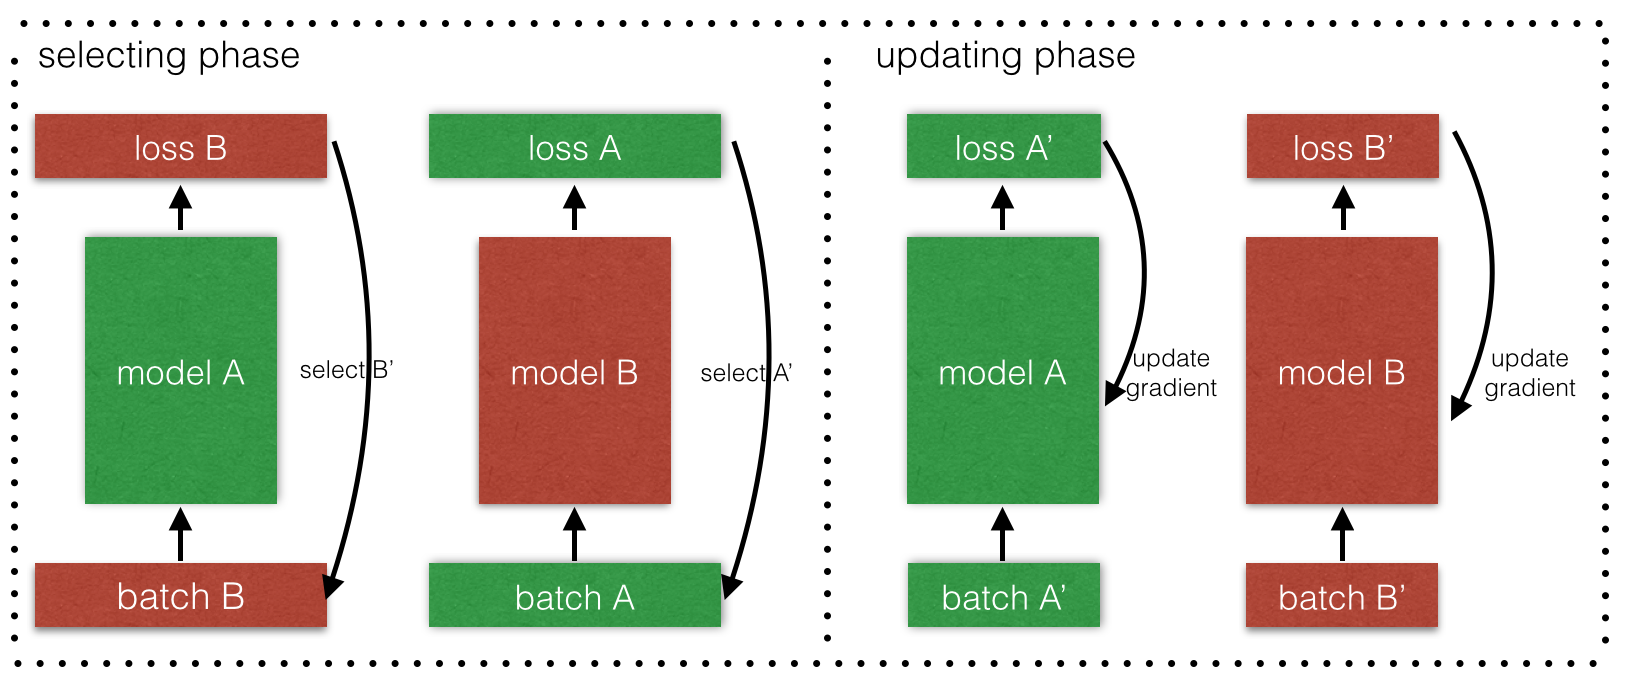
\includegraphics[width=14cm]{figures/coteaching.png}
    \caption{Our proposed solution.}
    \label{fig:framework}
\end{figure}


\section{Experiments}
\subsection{Data Preparation and Configuration}

Specify how to process the data, how to evaluate the performance (e.g., mAP).
\begin{table}[ht]
    \centering
    \begin{tabular}{l|c|c|c}
    \hline
     Dataset & \#train & \#test & \#Category\\
    \hline
    MNIST& 60,000 & 10,000 & 10  \\
    CIFAR-10& 50,000 & 10,000 & 10 \\
    \hline
    \end{tabular}
    \caption{Summary of datasets.}
    \label{tab:dataset}
\end{table}

\subsection{Implementation}
Give a figure to illustrate your implementation, then detail each parts.

\subsection{Results}
Present the results, both qualitatively (visualize) and quantitatively (specific numbers)..
Analyze the results
\subsection{Discussion}
Strengths and weakness in your method.

\section{Conclusion}
In this project, we ...

\section{Group Information}
\begin{table*}[ht]
    \centering
    \begin{tabular}{l|c|c|c}
    \hline
     Member & Student ID & Email & Contribution\\
    \hline
    Maximilian Fruehauf& Axx & e0445541@u.nus.edu & xxx \\
    David Drews& Axx &e0454245@u.nus.edu & xxx  \\
    Choo Wen Xin& A0160465H & e0053347@u.nus.edu & xxx  \\
    \hline
    \end{tabular}
    \caption{Group member information.}
    \label{tab:dataset}
\end{table*}
\bibliographystyle{plain}

\bibliography{references}
 
\end{document}




